ITAPS uses the information flow through a mesh-based simulation to
guide the development of interoperable geometry, mesh and solution
field components.  While the information flow is modeled using the
requirements of a mesh-based PDE solver, the resulting components are
general enough to provide the infrastructure for a variety of other
tools including pre/post-processing of discrete data, mesh and
geometry manipulation, and error estimation.  A simulation's
information flow, depicted in Figure~\ref{fig:infoFlow}, begins with a
problem definition.  Described in more detail in
Section~\ref{sec:probDef}, the problem definition
%kkc 050613 includes the domain of the problem, 
%kkc 050613 the governing
%kkc 050613 mathematical form (PDEs, variational principle, etc) and any
%kkc 050613 parameters associated with the governing mathematics.  
consists of a description of the simulation's geometric and temporal
domain annotated by {\it attributes} designating mathematical model
details and parameters.
%kkc 050613 moved to 2.1 For example, a PDE solver may annotate the geometry with the
%kkc 050613 moved to 2.1 mathematical form governing the simulation (PDEs, variational
%kkc 050613 moved to 2.1 principle, etc) and any parameters associated with the governing
%kkc 050613 moved to 2.1 mathematics.  Other problem definitions (e.g. data analysis, adaptive
%kkc 050613 moved to 2.1 loops, mesh optimization, etc) may require additional or different
%kkc 050613 moved to 2.1 annotations.  
%Geometry representation %kkc 050613,  management 
%and attribute annotation form the central pieces of the problem definition.
%kkc 050613 Following problem definition
In the next stage of the information flow, mesh-based simulation
procedures approximate the PDEs by first decomposing the geometric
domain into a set of piecewise components, {\it the mesh}, and then
approximating the continuous PDEs on that mesh using, for example,
finite difference, finite volume, finite element, or partition of unity
methods.  Once the domain and PDEs are discretized, a number of
different methods can be used to solve the discrete equations and
visualize or otherwise interrogate the results.  Simulation automation
and reliability often imply feedback of the PDE discretization
information back to the domain discretization (i.e. in adaptive
methods) or even modification of the physical domain or attributes
(e.g., design optimization).  
%lad not sure this is useful info here
%Even when ITAPS components are not used to
%write the actual PDE solver, these components can be used to marshal
%information from the PDE solver back to the problem definition or
%domain discretization as part of a larger application such as an
%optimization or adaptive process.
%lad i don't think the following section adds anything at this point in
%    the text
%Information in the domain discretization, discussed in
%Section~\ref{sec:domainDisc}, is managed by mesh generation and mesh
%representation.  The geometry and mesh representations synergisticly
%form a conduit providing information to the other areas of the
%simulation: PDE discretization, solution and field interrogation.
%(Section~\ref{sec:pdeDisc}).   
The following sections present ITAPS' %kkc 050613 definition 
model of the information
flow in mesh-based simulations; these sections also introduce the
concepts of geometry, mesh and solution fields used to define ITAPS'
interoperable interfaces.

%\begin{figure}
%\begin{center}
%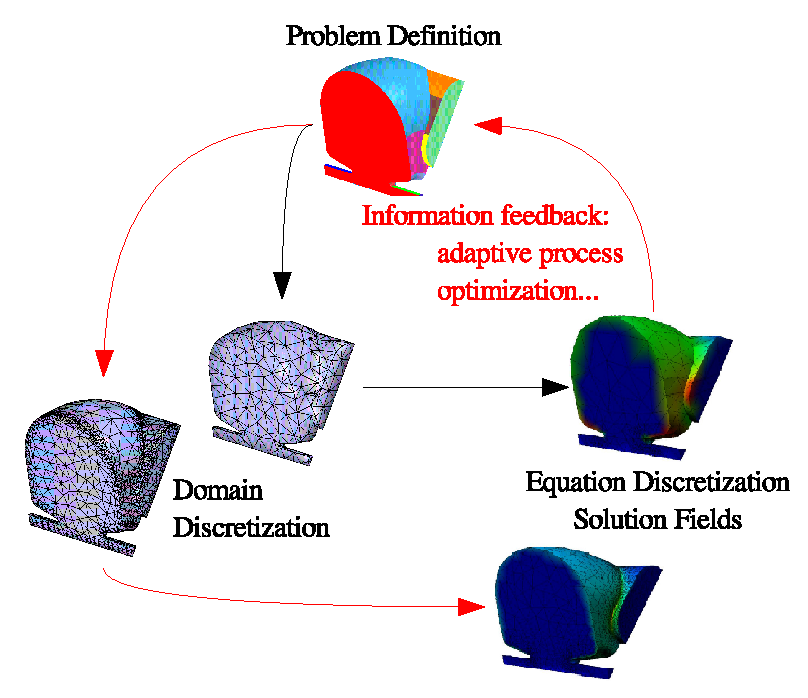
\epsfig{file=information_flow.eps,width=10cm}
%\caption{The information flow in a mesh-based simulation begins with
%a problem definition and continues through the domain and PDE
%discretizations.  Dynamic processes, such as solution adaptation and
%design optimization, require components capable of feeding information
%back to other parts of the information flow.}
%\label{fig:infoFlow}
%\end{center}
%\end{figure}

%kkc In mesh-based analysis procedures the PDEs are solved approximately
%kkc through a double discretization process in which the problem's
%kkc physical domain is discretized into a set of piecewise components
%kkc (e.g. a mesh) and the PDEs to be solved are discretized over the mesh
%kkc in an appropriate manner. The discretizations of the PDEs over the
%kkc mesh are assembled into a fully discrete system that is solved. The
%kkc result of this process yields the construction of a set of discretized
%kkc solution fields. Methods covered by such approaches include finite
%kkc difference, finite volume, finite element, boundary element and
%kkc partition of unity (so-called meshfree) methods.

\subsection{Problem Definition}\label{sec:probDef}

%kkc To qualify the operations and information involved in executing a
%kkc mesh-based simulation, we begin with a qualification of the problem
%kkc definition which includes:
%CFO-G We begin with a problem definition that qualifies the information (LAD
%CFO-G ???? WHAT DOES THIS MEAN?) and operators required by a mesh-based
%CFO-G simulation.  The problem definition includes:
%CFO-G 
%CFO-G Here's my swing at this one:
%kkc 050613 I like CFOG's sentence.
%% To identify the operations and information needed by a mesh-based
%% simulation, we begin with a problem definition containing:

%% \begin{itemize}
%% %I think this is more direct (cfog).  Also, moving it up puts the domain
%% %stuff together at the end for a nice transition to that topic...
%% \item The domain over which the simulation is to be performed. For the
%% classes of simulations being considered here the domain includes a
%% spatial component that is one-, two-, or three-dimensional and can
%% also include a temporal component if the solution changes with time.

%% %kkc 050613 \item The mathematical equations describing the physical processes to be
%% %kkc 050613 simulated (written as PDEs, variational principles, weak forms, etc).
%% %\item The mathematical form governing the simulation (e.g., PDEs,
%% %variational principles, weak forms).

%% \item Specification of %kkc 050613 parameters, referred to as 
%% physical {\it attributes} such as the %associated with including the governing
%% mathematical equations, material properties, forcing functions,
%% boundary conditions, and initial conditions.
%% \end{itemize}

%kkc 050613 rewrite the above description as single paragraph
To identify the operations and information needed by a mesh-based
simulation, we begin with a problem definition containing the {\it
domain} over which the simulation is to be performed and {\it
attributes} describing the problem that is to be solved.  For the
classes of simulations being considered here, the domain includes a
spatial component that is one-, two-, or three-dimensional and can
also include a temporal component if the solution changes with time.
To support a numerical simulation, the domain representation must be
able to support any geometry interrogation and/or modification
required by mesh generators and simulations, and the association of
mathematical and physical {\it attributes} with the geometry.  {\it
Attributes} specify the mathematical information required to solve a
particular problem.  This information includes, e.g., equations,
material properties, forcing functions, boundary conditions, and
initial conditions.  For example, a PDE solver may require a domain
definition annotated with the mathematical form governing the
simulation (PDEs, variational principle, etc) and any parameters
associated with the governing mathematical equations.  Other problem
definitions e.g., data analysis, adaptive loops, mesh optimization,
etc., may require additional or different attributes.

\begin{figure}
\begin{center}
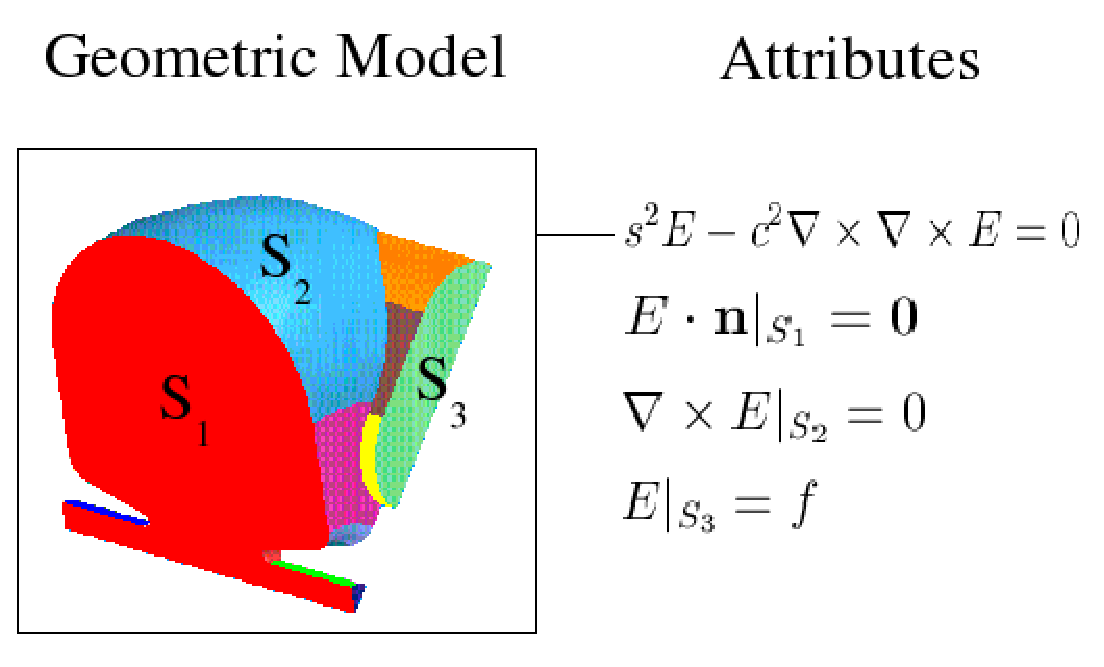
\epsfig{file=problem_description.eps,width=9cm}
\caption{The problem definition includes a geometric description of the domain
as well as attributes associated with geometric entities.  These attributes
are used to define the mathematical problem, its parameters and any other 
information needed by the simulation process.}
\label{fig:probDef}
\end{center}
\end{figure}

%\begin{itemize}
%\item Support the construction of a mesh that represents the domain
%discretization used in the simulation.

%\item Support any geometry interrogation required.
%\item any geometry interrogation and/or modification required by
%mesh generators and simulations, and

%\item the association of the physical and mathematical
%attributes with the geometry. %kkc ? mesh. cfog: concur

%\item Support the domain evolution in the cases where the domain
%changes as part of the solution process.
%\end{itemize}

\subsubsection{Geometric Domain}

%lad not sure this adds significantly to the bullets above
%lad Geometry interrogation and management supports the information flow at
%lad numerous points in a simulation.  Mesh generation and adaptation in
%lad particular rely upon geometric queries when discretizing the domain
%lad boundaries.  Physical models and discretizations require the
%lad information provided by attributes associated with the geometry.  For
%lad example, boundary conditions, initial conditions and constitutive
%lad models constitute information that can associated with the geometry.

%cfog What follows is a massive reordering of a couple of paragraphs to
%cfog avoid the issue, noted by Lori and/or Kyle, that we seem to be
%cfog dismissing CGM, image data, etc a bit too hastily.  Mostly I've
%cfog changed order, with some inevitable cleanup following.

%kkc 050613 I think we are still dismissing it, just less obviously now. (grep: more lines!)
%           The only way to support, for example, implicit or level set surfaces
%           with the current description would be to tesselate them 
%           and then compute a topological decomposition
%           of the triangulated surface (using methods referenced below).
%           The way I see it, non-b-rep geometry data is going to become more
%           important, not less.  The computer graphics folk seem to be heading
%           toward subdivision surfaces in a big way.  Again, those *could* be
%           used to construct a topological model; thus doing away with all the
%           nice features of subdivision methods.  Also, there have been many 
%           recent papers in siggraph (and such) on implicit surface modeling
%           Again, we only address this through firey hoops and assigning work 
%	    to others (hey, you come up with the algorithms).
%	    
%	    Why am I chewing on this bone?  Modeling biological and geophysical
%           processes (to name two up and comming cases) involve geometries
%           whose b-rep models are not available.  You can ask, but I am not sure
%           you will get an answer.  In EB applications we are seeing a lot
%           of implicit and level set surface definitions being used without needing
%	    the b-rep to generate the EB information.  These
%           representations are also useful for image data, MRI,CAT, and PET imaging.
%           Siesmograph modeling of subsurface features come in some form of
%           volume representation.  GIS data may come in triangulations
%           but I submit that any attempted topological decomposition of the Rockies would
%           be more confusing than a triangulation, not less.
%           
%           Is relying on the concept of a b-rep really a good long term strategy?
%           Not that I have an alternative yet, mind you, but maybe it is too
%           close to specifying an implementation... 
%	    YES, it is too late to bring this up. I only thought about it while editing the paper.
%	    
%	    
%	    At any rate, I think we need to have some answer; even if that answer
%	    is to convert the implicit/subdivision/voxel/etc data into a tesselated surface
%           which is then fed into a topology extraction algorithm.

%rev 1653:
%% Supporting geometry interrogation, modification and attribute
%% association requires a complete and flexible interface to the spatial
%% domain definition.  There are multiple approaches for defining the
%% spatial domain.  Computer aided design (CAD), image data and
%% cell-based (mesh-based) are among the most common geometry sources.
%% Each of these sources has one or more representational
%% forms. Historically, CAD systems use boundary representations. Image
%% data use a volumetric form such as voxels or octrees.  For cell-based
%% geometry, a variety of implicit and explicit boundary or volumetric
%% representations have been used.  Except in cases of image data and
%% when all aspects of the simulation process can be effectively defined
%% in terms of volumetric representations (e.g.  constructive solid
%% geometry, level sets, etc), it is generally accepted that the use of a
%% boundary representation is well suited for the spatial domain
%% definition.

%% WE JUST DISMISSED IMAGE, CSG, AND OTHER FORMS OF NON-BREP GEOMETRY.
%% DO WE REALLY WANT TO DO THAT...

%% A boundary representation (b-rep) consists of a collection of {\it
%% geometric entities}.  In this context, geometric entities are volumes,
%% surfaces, curves and points that collectively define a bounded portion
%% of three-dimensional space~\cite{mort97}; this bounded subset is
%% referred to as the {\it geometric model}.  There is substantial
%end rev 1653

Supporting geometry interrogation, modification and attribute
association requires a complete and flexible interface to the spatial
domain definition.  We consider {\it geometric models} that are subsets
of three-dimensional space bounded by a collection of {\it geometric
entities} (points, curves, surfaces, and volumes)~\cite{mort97}.  There
is substantial computer-aided design literature on various domain
representations.  Boundary representations (b-reps), which are the
most common geometric representation in CAD systems, are particularly
well-suited for geometric models as we define them.  Other domain
representations are also possible, including constructive solid
geometry; discrete (mesh-based) representations; and image data
(typically in the form of voxels or octrees).

For our purposes, details of how the geometric shape of the domain is
represented are immaterial.  We focus instead on the topological
abstractions to represent the geometric entities.  Topologically 3-, 2-,
1- and 0-dimensional entities are referred to as regions, faces, edges
and vertices, respectively.  Vertices form the boundaries of edges
(except in periodic edges, whose boundary set is null), edges bound
faces and faces are used to define regions.  The topological structure
of the geometric model is completely described by these entities and
their adjacencies.  The actual geometric information associated with a
geometric model entity, its shape, can be thought of as an attribute of
the entity.

The effective interaction of multiple domain definition sources
requires the definition of abstract interfaces that use information
that is common to all of them: that is, their topological entities.
%The ability to interact with
%topological entities provides an effective means to develop abstract
%interfaces allowing the easy integration to multiple domain definition
%sources.  
The ability to generalize these interfaces is further
enhanced by the fact that the geometry shape information needed by
most simulation procedures consists of pointwise interrogations that
can be easily answered in a method independent of the modeler shape
representation.  
%lad not sure what this adds
%lad The developers of CAD systems support geometry-based
%lad applications through general APIs.  These geometric modeling APIs have
%lad been successfully used to developed automate finite element modeling
%lad processes\cite{BeWa04,ShGe92}.

%lad too much detail
%lad An important consideration in the selection of a boundary
%lad representation is its ability to represent the classes of domain
%lad needed. In the case of numerical simulations the domains to be meshed
%lad can be general combinations of 0-, 1-, 2- and 3-D entities in general
%lad configurations. Figure~\ref{fig:non-man-model} shows a typical
%lad analysis domain that may be used for the structural analysis of a
%lad portion of a piping system. The analysis domain is an idealization
%lad where portions of the pipes are idealized by beams, the support
%lad bracket idealized by a plate and a full 3-D solid used for the pipe
%lad juncture.  The representation of such geometric domains, as
%lad well as others like multi-material domains, are referred to as a
%lad non-manifold boundary representations \cite{GuCh90,We88}. In the case
%lad of non-manifold models the representation must indicate how
%lad topological entities are used by bounding higher order entities. For
%lad example, each side of a face may be used by a different
%lad region. Therefore, faces have two uses. Another terminology for the
%lad use of a topological entity by higher order topological entities is
%lad co-entities \cite{Ta00}.

%% \begin{figure}
%% \begin{center}
%% \begin{pspicture}(-1,0)(11,6)
%% \rput(5,3){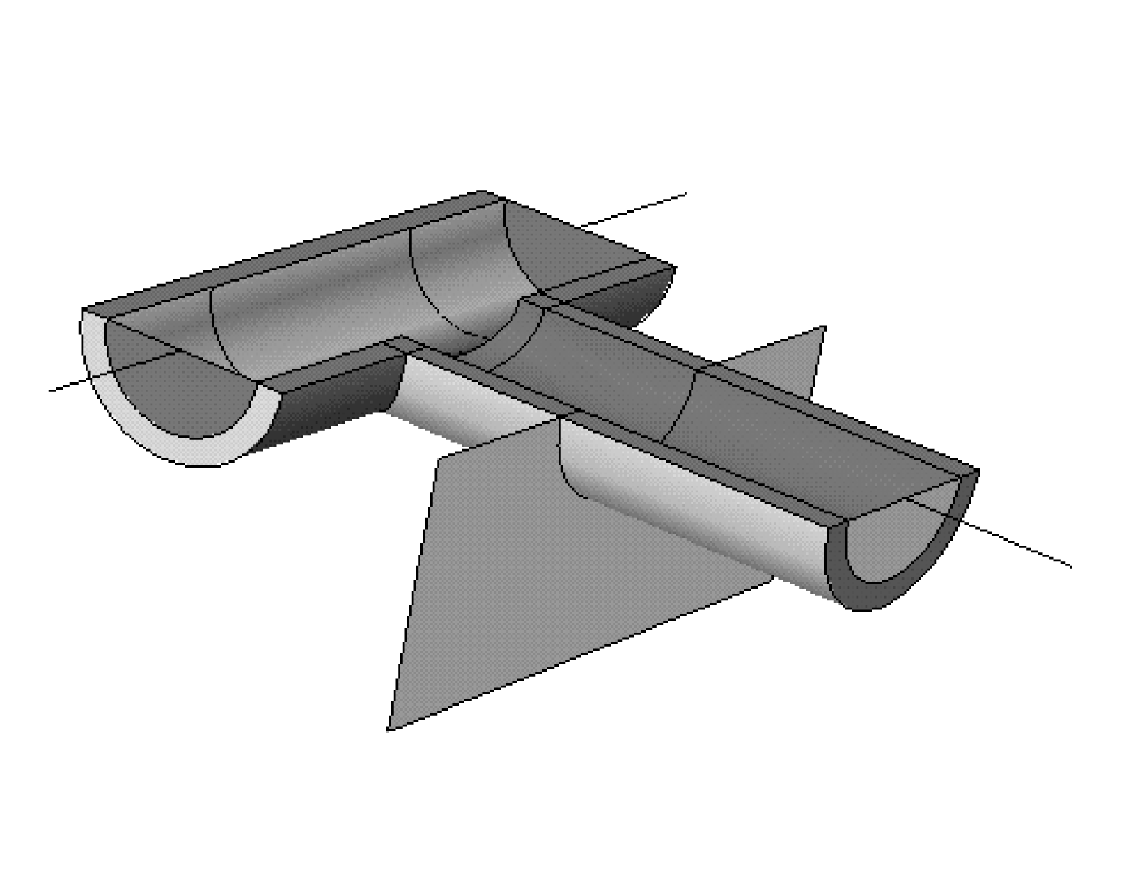
\epsfig{file=non-man-model.ps,width=9cm}}
%% \rput(4.2,.7){\makebox(0,0)[l]{\footnotesize support bracket (plate)}}
%% \rput(9.1,2.2){\makebox(0,0)[l]{\footnotesize pipe (beam)}}
%% \rput(6.,5.2){\makebox(0,0)[l]{\footnotesize pipe (beam)}}
%% \rput(1,3.2){\makebox(0,0)[r]{\footnotesize pipe (beam)}}
%% \rput(2.2,4.8){\makebox(0,0)[r]{\footnotesize junction (3-D solid)}}
%% %\psgrid
%% \end{pspicture}
%% \caption{A typical problem domain for the structural analysis of a piping system may use
%% geometric entities of different topological dimension for various
%% portions of the domain.  In this case, portions of the pipes are
%% idealized by beams, the support bracket idealized by a plate and a
%% full 3-D solid used for the pipe juncture.}
%% \end{center}
%% \end{figure}\label{fig:non-man-model}
%kkc Figure 1. Example of a non-manifold model used in simulation.

%ARE THE FOLLOWING TWO PARAGRAPHS REALLY RELEVANT TO THE INFORMATION FLOW????

%lad too much detail
%lad Geometric modeling systems maintain tolerance information on how
%lad numerically well the entities fit together.  This is necessitated by
%lad the fact that to function properly geometric modeling systems must
%lad employ finite tolerances.  The algorithms and methods within the
%lad geometric modeling system use the tolerance information to effectively
%lad define and maintain a consistent representation of the geometric
%lad model. (What many geometry-based applications have referred to as
%lad dirty geometry is caused by a lack of knowledge and proper use of the
%lad tolerance information \cite{BeWa04}.)

%lad Sometimes the only available domain representation is a mesh. Often it
%lad is still desirable to construct a high level topological
%lad representation of the problem domain. The process of constructing, or
%lad updating, the topological entities representing the domain geometric
%lad model is focuess on determining the appropriate subsets of the mesh to
%lad assocaiate with the model regions, faces, edges and vertices.
%kkc avoid ``mesh entities'' before introduction in the next section
%kkc is focused on determining the appropriate
%kkc sets of mesh regions, faces, edges, and vertices to associate with the
%kkc model regions, faces, edges and vertices respectively. 
%lad Algorithms to do this based on mesh based geometry and/or simulation
%lad contact or fracture information have been developed
%lad \cite{KrOr01,PaOr02,WaKo04}.  Once the model topology has been set,
%lad the geometric shape information can be defined in terms of the mesh,
%lad or can be made higher order \cite{CiOr00,OwWh01}.

%% kkc 050613 got rid of the next section since it has been supplanted by discussions
%%            in the problem definition introduction and geometric domain and attribute sections

%% \subsubsection{Governing Mathematics}

%% WE SHOULD DISCUSS SPECIFICIATION OF THE GOVERNING MATHEMATICS HERE.
%% WHAT IS THERE TO SAY?
%% HOW ABOUT :

%% LAD: I DON'T THINK THIS IS QUITE THE RIGHT INFORMATION AND I'M NOT HAPPY WITH
%% ATTRIBUTES BEING EVERYTING INCLUDING THE PDE.. IT SEEMS LIKE THERE SHOULD BE
%% SOME DISTINCTION - SO I WOULD LIKE TO TALK ABOUT BC, IC HERE - THEY ARE INTRINSIC
%% TO THE PDE - I WOULD WANT TO TALK ABOUT PARAMETERS BELOW - MATERIAL PROPERTIES
%% FOR EXAMPLE

%% The second aspect of problem definition are the governing mathematics.
%% A classical simulation tool's governing equations were built directly
%% into the structure and information flow of a code.  For example, a
%% time dependent PDE solver usually had a ``timestepping'' loop
%% surrounding the specific discretizations for the spatial part of the
%% PDE system.  Simulation frameworks often provide provide general
%% operators for discretizing PDEs that can be organized into codes
%% solving a particular problem~\cite{BrLa97,overtureTR,BeSh99}. Even
%% higher level approaches exist where interpreted languages or even
%% graphical interfaces are used to specify the high-level problem
%% definition.  Additional tools then translate this high level
%% specifiction into executable code by automatically assembling the
%% software components implied by the problem
%% definition~\cite{virtCell,pdeLab}.  ITAPS' component approach
%% addresses the first case, pre-exist information flow, by providing
%% common interfaces to information required by simulation codes.
%% Classical simulation tools can use ITAPS components to enhance or
%% expand their problem definitions without massive code development.
%% Simulation frameworks can use ITAPS tools to both expand the range of
%% problems they support as well as provide interfaces to their own
%% technology for use by other applications.  Finally, providing an
%% abstract interface to the information in the problem definition will
%% will allow high level interfaces access to alternative technologies
%% for domain representation and attribute association.  
%% UGH!!! STILL NOT HAPPY WITH THIS

\subsubsection{Attributes}
%kkc An examination of the properties of analysis attributes indicates they
%kkc are tensorial quantities \cite{BeSo83} that must be defined with
%kkc respect to a coordinate system. Generalized structures and methods can
%kkc define analysis attributes and associate them geometric model entities
%kkc\cite{OBSh02}.
Analysis {\it attributes} are information
associated with specific geometric entities in
the domain definiton.  In a PDE solver, these attributes include
the PDEs and initial conditions associated with a model region,
boundary conditions associated with boundary faces, and source terms
located within a model region.  Some attributes may be tensor-quantities %kkc 050613required by the problem definition and 
defined in various coordinate systems leading to the need for coordinate transformations
that allow other parts of the simulation process to access the data.
For example, a source term in the governing PDE is associated with a
geometric location in space and could be expressed using polar,
spherical or cartesian coordinates depending on the discretization.
%kkc 050613 not sure what else to say about attributes...

%One example could
%be a vector source term in the governing PDEs that is defined in
%spherical polar coordinates.  This source term would need to be
%transformed to Cartesian coordinates prior to use in a PDE
%discretization expressed in Cartesian coordinates.  
%kkc 050613 Generalized
%kkc 050613 structures and methods can define analysis attributes and associate
%kkc 050613 them with geometric model entities\cite{OBSh02}.  

\subsection{Domain Discretization}\label{sec:domainDisc}

The mesh is a piecewise decomposition of the space/time domain.  It is
common to employ different discretizations for the spatial and temporal
domains.  Because the definition of the spatial mesh is typically the
more complex of the two, it is the focus of this discussion.  In
addition to the case where a single mesh covers the entire geometric
(spatial) domain, we also consider cases where more than one mesh is
associated with a domain.  For example, in hybrid meshing approaches,
the domain is decomposed first into a set of sub-domains that may be
meshed using different meshing strategies.  Also, different full
geometry meshes can be used during different stages of the numerical
solution, as in the case of multilevel or adaptive methods.  In each of
these cases, the meshes can be associated with the underlying geometric
domain so that any changes made to the domain propagate properly to all
meshes.

\begin{figure}
\begin{center}
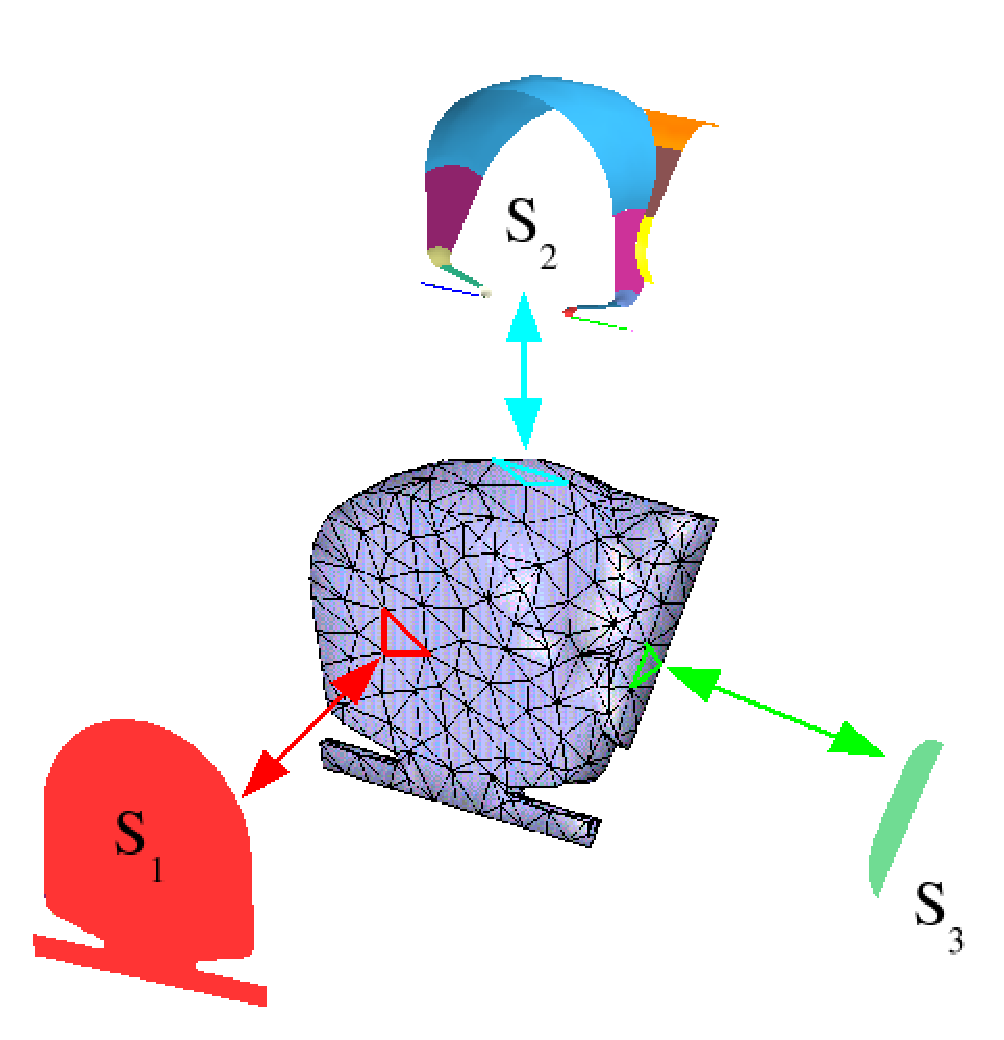
\epsfig{file=domain_discretization2.eps,width=8cm}
\caption{The domain discretization is a piecewise decomposition of the domain; usually a mesh.  Entities in the mesh (Vertices, Edge, Faces, and Regions) can
be associated with entities in the geometric model.  This association is referred to as ``classification'' of mesh entities on model entities.  Reverse classification associates model entities with mesh entities residing on that portion of the model.}
\label{fig:domainDisc}
\end{center}
\end{figure}

While different discretization approaches place different requirements
on the mesh and mesh entities, in general the mesh is required to
\begin{itemize}
\item have the appropriately defined union of the mesh
entities represent the domain of interest,
\item maintain, or have access to, the geometric shape information
needed for processes such as differentiation and integration,
\item support the PDE discretization process over the mesh entities, and
\item maintain relationships of the mesh entities needed to support
the assembly of the complete discrete system and construction of the
solution fields.
\end{itemize}

Meshes can take many different forms, the simplest of which is
a conforming mesh where the intersections of
two mesh entities is null and the intersections of their closure is
either null or the closure of a common boundary mesh entity (face,
edge or vertex). Other mesh forms include non-conforming meshes,
hierarchical, patch-based meshes, or overlapping meshes.
%lad where
%lad the intersections of the closure of two mesh entities is null, or
%lad different parts of the boundaries of the two mesh entities. Other mesh
%lad structures employ mesh patches that can interact in a variety of
%lad ways. Finally, other methods are defined in terms of overlapping
%lad regions (e.g. spheres or cubes). 
In each of these cases, there are
rules on how the mesh entities interact, how equation discretizations
are performed over them, and how the complete discrete system is
assembled.

%cfog Most of the following seemed to me to fit very well at the top of
%cfog the subsection.

%% THE FOLLOWING PARAGRAPH WAS MOVED FROM interface.tex TO HERE,
%% IT SHOULD BE WORKED INTO THIS SECTION

%% This domain must be decomposed into a set of mesh
%% entities. This process may employ a hierarchical decomposition of the
%% geometric domain. For example, the first level may decompose the
%% domain into a set of sub-domains that can be meshed using various
%% meshing strategies.  In particular, hybrid meshes consisting of
%% different component meshes can be used to discretize different
%% portions of the geometric domain, or different full geometry meshes
%% can be used during different stages of the numerical solution.  Each
%% of these meshes is associated with the full geometry domain so that
%% any changes made there propogate properly to the associated meshes.
%% Each mesh can be further decomposed into partitions for solution on a
%% massively parallel computer.

The geometric shape of the mesh entities is needed to support the
equation discretization process and can be effectively associated with
the topological entities defining the mesh. In many cases, this is
limited to the coordinates of the mesh vertices and, if they exist,
higher-order nodes associated with mesh edges, faces, or regions.  It
is also possible to associate other forms of geometric information
with the mesh entities, for example, associating Bezier curves and
surface control points with mesh edges and faces for use in {\it
p}-version finite elements \cite{LuSh02}.

It is possible to obtain mesh shape information by maintaining
an explicit link between mesh entities and a high-level description of
the geometric domain when it is available.  However, obtaining
information in this way is expensive and is often only used when
necessary.  Consider the case of mesh adaptation, the original domain
geometry must be used to ensure that the mesh approximates the
geometric domain to the same order of accuracy as the equation
discretization process approximates the continuous problem. For
example, as piecewise linear elements approximating curved portions of
the geometry are refined, the new mesh vertices must be placed on the
curved boundary, or as the polynomial order of an element is
increased, the geometric approximation of the closure of that entity
must be increased to the correct order.  If this high level geometric
information is not needed, for example, in the case of fixed mesh
simulations, it is typical to use only geometric shape information
associated directly with the mesh entities.

The data model for the mesh must maintain an association with the
domain definition, the discretization functions, the assembled
discrete system and the solution fields. From the perspective of
maintaining its relationship to the geometric domain, the use of
mesh topological entities and their adjacency is ideal
\cite{BeSh97,DeOB01,Ta00}. In this manner it is possible to associate
the mesh entities to the domain entities to obtain needed attributes
and geometric information.  In other cases, using topological entities
is not ideal.  For example, when using partition of unity (so
called meshfree) methods, an octree, or some other spatially-based
structure, is more appropriate. In the case of structured meshes
maintaining an explicit list of mesh entities is unnecessary; instead
one can maintain the boundaries of the mesh patches augmented with the
rules of mesh patch interaction.

We refer to the association of the mesh with respect to the geometric
model as {\it classification} \cite{BeSh97,ShGe92}. In particular, the
mesh topological entities are classified with respect to the geometric
model topological entities upon which they lie as defined below.

{\bf Definition: Classification} - {\it The unique association of mesh
topological entities of dimension $d_i$, $M^{d_i}_i$ to the
topological entity of the geometric model of dimension $d_j$,
$G^{d_j}_j$ where $d_i \leq d_j$, on which it lies is termed
classification and is denoted $M^{d_i}_i \sqsubseteq G^{d_j}_j$
where the classification symbol, $\sqsubseteq$,
indicates that the left hand entity, or set, is classified on the
right hand entity.}

{\bf Definition: Reverse Classification} - {\it For each model
entity, $G^d_j$ , the set of equal order mesh entities classified on that
model entity define the reverse classification information for that
model entity. Reverse classification is denoted as:}
\begin{equation}
RC(G^d_j) = \left\{ M^d_i | M^d_i \sqsubseteq G^d_j \right\}.
\end{equation}

The concept of mesh entity classification to a higher level model can
be extended to include additional levels of model decomposition. Two
important cases of this are parallel mesh partitions and structured
mesh partitions. In the cases when these partitions are
non-overlapping, the associations are obvious.  The concepts can be
extended to the case of overlapping partitions through the definition
of appropriate interaction rules for entities in the different models.

\subsection{Equation Discretization and the Definition of Solution Fields}\label{sec:pdeDisc}

The PDEs being solved are written in terms of dependent variables that
are functions of the space/time domain. Let the independent variables
of space be denoted ${\bf x}$, and the independent variable time be
denoted $t$.  For purposes of this discussion, let the set of
PDEs being solved be written in the form:

\begin{equation}
{\cal{D}}({\bf u}, \sigma) - f = 0
\end{equation}

where 
\begin{itemize}
\item $\cal{D}$ represents the appropriate differential operators,
\item $\bf{u} (\bf{x},t)$ represents one or more vector dependent variables,
\item $\sigma (\bf{x},t)$ represents one or more scalar dependent variables, and
\item $f (\bf{x},t)$ represents the forcing functions.
\end{itemize}
Note that the complete statement of a PDE problem must include a set
of boundary and, for time dependent problems, initial conditions.

In mesh-based PDE solvers, the dependent variables are discretely
represented over individual mesh entities or compact groups of entities,
either by direct operator discretization (e.g., difference equations) or
in terms of a set of basis functions. In both cases, this process
specifies a set of distribution functions defining how the discretized
variables vary over the mesh entities and a set of yet to be determined
multipliers, called degrees of freedom (DOF). The DOF can always be
associated with a single mesh entity while the distribution functions
are associated with one or more mesh entities.  Three common cases that
employ different combinations of interactions between the mesh entities,
the DOF, and the distributions are:
\begin{figure}
\begin{center}
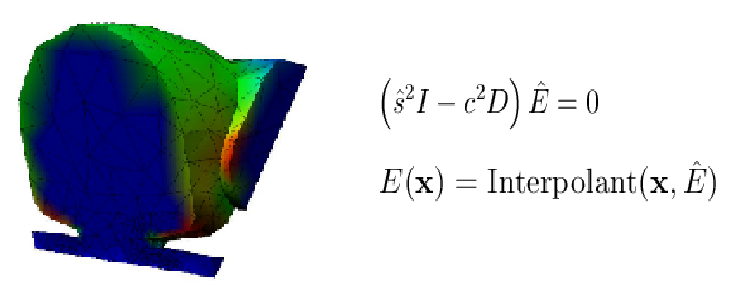
\epsfig{file=solution_fields.eps,width=8cm}
\caption{Solution fields provide access to simulation data and
discretizations.  In this example, $D$ is the discrete approximation
to the continuous system specified in the problem definition in
Figure~\ref{fig:probDef}.}
\label{fig:fields}
\end{center}
\end{figure}


%cfog:  I've inserted my own $0.02 here about the interpretation of
%cfog:  finite difference and finite volume methods.  Feel free to
%cfog:  change/debate my version as you see fit.

%kkc 050613 : thanks cfog, I concur with your changes.
\begin{description}
\item[{\it Finite difference methods.}]  In this case, the solution is 
represented by direct operator discretization: difference stencils are
written for all terms in the PDE.  These stencils are written in terms
of DOF that are the pointwise solution values for a compact collection
of mesh vertices.

\item[{\it Finite volume methods.}]  Finite volume methods compute the average
value of the solution in a set of control volumes that tesselate the
computational domain; these averages are the DOF.  Control volumes are
associated with mesh entities (vertices, edges, faces, or regions,
depending on the details of the scheme).  The distribution functions are
piecewise polynomials with discontinuities at control volume boundaries;
the coefficients of the polynomials are found using the DOF in
neighboring control volumes.


%cfog Mark:  I edited this paragraph a bit for length, considering that
%cfog it was longer than the finite difference and finite volume paras
%cfog combined.  I don't think I introduced any substantive errors in
%cfog the process, but it certainly bears checking.
\item [{\it Finite element methods.}]
Finite element distribution functions, referred to as shape functions,
are written over individual mesh entities, referred to as elements.  The
DOF represent values of the solution at particular points in the mesh
entity, refered to as nodes.  The shape functions associated with
neighboring elements can be made $C^m,~m \geq 0,$ continuous by having
common DOF associated with the shared lower-dimensional mesh entities.
In this case, the full set of DOF used by the element distribution
function can be associated with any of the mesh entities in the
closure of the mesh entity of the element.
\end{description}

Applying the discretization operation locally over the appropriate mesh
entities will produce a local contribution to the complete fully
discrete system.
%lad too much detail 
%lad The processes can be stated symbolically as:
%lad 
%lad \begin{equation}
%lad \cal{D} (\bf{D}^c, \bf{d}^c) - \bf{f}^c = 0 
%lad \end{equation}
%lad 
%lad where: 
%lad 
%lad \begin{itemize}
%lad \item $\cal{D}$ represents the discretized differential operators written in terms
%lad of appropriate distribution functions, $D^c$, over the domain of the
%lad contributor $C$ and $\bf{d}^c$ represents the vector of DOF associated with that
%lad contributor.
%lad 
%lad \item $\bf{f}^c$ represents the discretized representation of the known
%lad ``forcing functions'' and boundary conditions for that
%lad contributor.
%lad \end{itemize}
These can be combined to yield a discrete representation of the original
PDEs over the entire domain.
%lad that can be written as:
%lad 
%lad \begin{equation}
%lad \bf{k}^c \bf{d}^c = \bf{f}^c
%lad \label{eq:contrib_matrix}
%lad \end{equation}
%lad 
%lad where $\bf{k}^c$ is a matrix of parameters for contributor $C$ that multiple the
%lad vector of DOF associated with that contributor, $\bf{d}^c$.
%lad 
The construction of the system contributors can be controlled by the
appropriate traversal of information in the high-level problem
definition (e.g., the geometric domain), or at a level above the mesh
such as the mesh patch level for structured methods.

Note that the solution fields represent the variations of the tensor
variables over the domain of the problem. These fields
must be maintained in a form that is useful for queries
and manipulation as needed.  These manipulations include
the transfer of the fields to other meshes during a 
multiphysics analysis step, or to maintain the description
of the mesh on an adapted field.  Another common function that fields must
support is the construction of new fields through operations
that project the data onto new distributions with higher order
continuity, combine with other fields, etc..

%LAD NOT SURE THIS SECTION IS NECESSARY FOR INFORMATION FLOW
%lad \subsection{Discretized System Construction and Solution}
%lad 
%lad The relationship of the contributor level discretization given in
%lad (\ref{eq:contrib_matrix})
%lad to the complete discrete system is dictated by contributor level
%lad mappings that ``map'' the contributor level DOF to the
%lad ``assembled'' vector of the DOF for the complete system, $\bf{d}$. The
%lad process of constructing the complete system from the contributors is
%lad referred to as the assembly process. Symbolically the complete
%lad discrete system can be written as:
%lad 
%lad \begin{equation}
%lad \bf{K} \bf{d} = \bf{F}
%lad \end{equation}
%lad 
%lad where
%lad 
%lad \begin{itemize}
%lad \item $\bf{K}$ is a system level matrix of parameters.
%lad \item $\bf{d}$ is the complete vector of DOF 
%lad \item $\bf{F}$ is the complete right hand side vector.
%lad \end{itemize}
%lad 
%lad Symbolically the relationship between the contributor level and system
%lad level matrices and vectors can be depicted as:
%lad 
%lad \begin{equation}
%lad \bf{d} ~=~ A^{N_c}_{c=1}(\bf{d}^c),~K~=~A^{N_c}_{c=1}(\bf{k}^c),~\bf{F}~=~A^{N_c}_{c=1}(\bf{f}^c)
%lad \end{equation}
%lad 
%lad where 
%lad \begin{itemize}
%lad \item $N_c$ is the number of contributors in the complete system
%lad \item $A^{N_c}_{c=1}$ indicates an assembly operator that is applied to each
%lad contributors contributions and properly maps it to the complete
%lad discrete system.
%lad \end{itemize}
%lad 
%lad There are a variety of specific representational forms for the
%lad complete systems matrices.  The specific form used is function of the
%lad methods used to perform the computationally intensive process of
%lad solving the discrete system to determine the values of the system DOF.
%lad The global algebraic equations are solved to produce the values of the
%lad system DOFs. Once the system level DOF are determined, the mappings
%lad between the contributor level and system level DOF can be used to
%lad complete the specification of the solution fields.


% LocalWords:  ITAPS interoperable PDEs KKC meshfree PDE TSTT's
